\documentclass[tikz]{standalone}

% \usepackage{tikz}

\begin{document}

\newcommand{\PolygonInit}{

\coordinate (A) at (0.1802,0.8712);
\coordinate (B) at (0.2573,0.7795);
\coordinate (C) at (0.0331,0.6281);
\coordinate (D) at (0.2457,0.6223);
\coordinate (E) at (0.2806,0.5088);
\coordinate (F) at (0.3723,0.6136);
\coordinate (G) at (0.3621,0.3996);
\coordinate (H) at (0.4306,0.3297);
\coordinate (I) at (0.5266,0.3195);
\coordinate (J) at (0.5630,0.0677);
\coordinate (K) at (0.8629,0.2103);
\coordinate (L) at (0.9401,0.5189);
\coordinate (M) at (0.7086,0.4942);
\coordinate (N) at (0.5892,0.6529);
\coordinate (O) at (0.6693,0.8014);
\coordinate (P) at (0.3985,0.9382);

\coordinate (Q) at (0.6,0.4);
\coordinate (R) at (0.6,0.2);
\coordinate (S) at (0.8,0.2);
\coordinate (T) at (0.8,0.4);

\fill[blue, fill opacity = 0.5] (A)--(B)--(C)--(D)--(E)--(F)--(G)--(H)--(I)--(J)--(K)--(L)--(M)--(N)--(O)--(P)--cycle;
\draw[thick] (A)--(B)--(C)--(D)--(E)--(F)--(G)--(H)--(I)--(J)--(K)--(L)--(M)--(N)--(O)--(P)--cycle;

\fill[white] (Q)--(R)--(S)--(T)--cycle;
\draw[thick] (Q)--(R)--(S)--(T)--cycle;

\node at (0.4,0.8) {$P_1$};
\node at (0.7,0.3) {$P_2$};

\foreach \pt in {A,B,C,D,E,F,G,H,I,J,K,L,M,N,O,P,Q,R,S,T}{
	\draw[fill=black] (\pt) circle (0.25pt);
}
\useasboundingbox (-0.25,-0.1) rectangle (1.25,1.1);

}

\newcommand{\PolygonP}{

\coordinate (A) at (0.1802,0.8712);
\coordinate (B) at (0.2573,0.7795);
\coordinate (C) at (0.0331,0.6281);
\coordinate (D) at (0.2457,0.6223);
\coordinate (E) at (0.2806,0.5088);
\coordinate (F) at (0.3723,0.6136);
\coordinate (G) at (0.3621,0.3996);
\coordinate (H) at (0.4306,0.3297);
\coordinate (I) at (0.5266,0.3195);
\coordinate (J) at (0.5630,0.0677);
\coordinate (K) at (0.8629,0.2103);
\coordinate (L) at (0.9401,0.5189);
\coordinate (M) at (0.7086,0.4942);
\coordinate (N) at (0.5892,0.6529);
\coordinate (O) at (0.6693,0.8014);
\coordinate (P) at (0.3985,0.9382);

\coordinate (Q) at (0.6,0.4);
\coordinate (R) at (0.6,0.2);
\coordinate (S) at (0.8,0.2);
\coordinate (T) at (0.8,0.4);

\fill[blue, fill opacity = 0.5] (A)--(B)--(C)--(D)--(E)--(F)--(G)--(H)--(I)--(J)--(K)--(L)--(M)--(N)--(O)--(P)--cycle;
\draw[thick] (A)--(B)--(C)--(D)--(E)--(F)--(G)--(H)--(I)--(J)--(K)--(L)--(M)--(N)--(O)--(P)--cycle;

\node at (0.4,0.8) {$P_1$};

\foreach \pt in {A,B,C,D,E,F,G,H,I,J,K,L,M,N,O,P}{
	\draw[fill=black] (\pt) circle (0.25pt);
}
\useasboundingbox (-0.25,-0.1) rectangle (1.25,1.1);

}

\newcommand{\ConvexHull}{

\coordinate (A) at (0.1802,0.8712);
\coordinate (B) at (0.2573,0.7795);
\coordinate (C) at (0.0331,0.6281);
\coordinate (D) at (0.2457,0.6223);
\coordinate (E) at (0.2806,0.5088);
\coordinate (F) at (0.3723,0.6136);
\coordinate (G) at (0.3621,0.3996);
\coordinate (H) at (0.4306,0.3297);
\coordinate (I) at (0.5266,0.3195);
\coordinate (J) at (0.5630,0.0677);
\coordinate (K) at (0.8629,0.2103);
\coordinate (L) at (0.9401,0.5189);
\coordinate (M) at (0.7086,0.4942);
\coordinate (N) at (0.5892,0.6529);
\coordinate (O) at (0.6693,0.8014);
\coordinate (P) at (0.3985,0.9382);

\coordinate (Q) at (0.6,0.4);
\coordinate (R) at (0.6,0.2);
\coordinate (S) at (0.8,0.2);
\coordinate (T) at (0.8,0.4);

\fill[green, fill opacity = 0.25] (A)--(C)--(J)--(K)--(L)--(O)--(P)--cycle;
\draw[thick] (A)--(C)--(J)--(K)--(L)--(O)--(P)--cycle;

\node at (0.5,0.5) {$A$};

\foreach \pt in {A,B,C,D,E,F,G,H,I,J,K,L,M,N,O,P,Q,R,S,T}{
	\draw[fill=black] (\pt) circle (0.25pt);
}
\useasboundingbox (-0.25,-0.1) rectangle (1.25,1.1);
}

\newcommand{\Trous}{

\coordinate (A) at (0.1802,0.8712);
\coordinate (B) at (0.2573,0.7795);
\coordinate (C) at (0.0331,0.6281);
\coordinate (D) at (0.2457,0.6223);
\coordinate (E) at (0.2806,0.5088);
\coordinate (F) at (0.3723,0.6136);
\coordinate (G) at (0.3621,0.3996);
\coordinate (H) at (0.4306,0.3297);
\coordinate (I) at (0.5266,0.3195);
\coordinate (J) at (0.5630,0.0677);
\coordinate (K) at (0.8629,0.2103);
\coordinate (L) at (0.9401,0.5189);
\coordinate (M) at (0.7086,0.4942);
\coordinate (N) at (0.5892,0.6529);
\coordinate (O) at (0.6693,0.8014);
\coordinate (P) at (0.3985,0.9382);

\coordinate (Q) at (0.6,0.4);
\coordinate (R) at (0.6,0.2);
\coordinate (S) at (0.8,0.2);
\coordinate (T) at (0.8,0.4);

\fill[red, fill opacity = 0.25] (A)--(B)--(C)--cycle;
\draw[thick] (A)--(B)--(C)--cycle;

\fill[red, fill opacity = 0.25] (C)--(D)--(E)--(F)--(G)--(H)--(I)--(J)--cycle;
\draw[thick] (C)--(D)--(E)--(F)--(G)--(H)--(I)--(J)--cycle;

\fill[red, fill opacity = 0.25] (L)--(M)--(N)--(O)--cycle;
\draw[thick] (L)--(M)--(N)--(O)--cycle;

\node at (0.1709,0.7677) {\tiny $B_1$};
\node at (0.3009,0.4416) {\tiny $B_3$};
\node at (0.7272,0.6228) {\tiny $B_2$};

\foreach \pt in {A,B,C,D,E,F,G,H,I,J,K,L,M,N,O,P}{
	\draw[fill=black] (\pt) circle (0.25pt);
}
\useasboundingbox (-0.25,-0.1) rectangle (1.25,1.1);
}

\newcommand{\TrouBUN}{

\coordinate (A) at (0.1802,0.8712);
\coordinate (B) at (0.2573,0.7795);
\coordinate (C) at (0.0331,0.6281);
\coordinate (D) at (0.2457,0.6223);
\coordinate (E) at (0.2806,0.5088);
\coordinate (F) at (0.3723,0.6136);
\coordinate (G) at (0.3621,0.3996);
\coordinate (H) at (0.4306,0.3297);
\coordinate (I) at (0.5266,0.3195);
\coordinate (J) at (0.5630,0.0677);
\coordinate (K) at (0.8629,0.2103);
\coordinate (L) at (0.9401,0.5189);
\coordinate (M) at (0.7086,0.4942);
\coordinate (N) at (0.5892,0.6529);
\coordinate (O) at (0.6693,0.8014);
\coordinate (P) at (0.3985,0.9382);

\coordinate (Q) at (0.6,0.4);
\coordinate (R) at (0.6,0.2);
\coordinate (S) at (0.8,0.2);
\coordinate (T) at (0.8,0.4);

\fill[red, fill opacity = 0.25] (A)--(B)--(C)--cycle;
\draw[thick] (A)--(B)--(C)--cycle;

% \fill[red, fill opacity = 0.25] (C)--(D)--(E)--(F)--(G)--(H)--(I)--(J)--cycle;
% \draw[thick] (C)--(D)--(E)--(F)--(G)--(H)--(I)--(J)--cycle;

% \fill[red, fill opacity = 0.25] (L)--(M)--(N)--(O)--cycle;
% \draw[thick] (L)--(M)--(N)--(O)--cycle;

\node at (0.1709,0.7677) {\tiny $B_1$};
% \node at (0.3009,0.4416) {\tiny $B_2$};
% \node at (0.7272,0.6228) {\tiny $B_3$};

\foreach \pt in {A,B,C,D,E,F,G,H,I,J,K,L,M,N,O,P}{
	\draw[fill=black] (\pt) circle (0.25pt);
}
\useasboundingbox (-0.25,-0.1) rectangle (1.25,1.1);
}

\newcommand{\TrouBDEUX}{

\coordinate (A) at (0.1802,0.8712);
\coordinate (B) at (0.2573,0.7795);
\coordinate (C) at (0.0331,0.6281);
\coordinate (D) at (0.2457,0.6223);
\coordinate (E) at (0.2806,0.5088);
\coordinate (F) at (0.3723,0.6136);
\coordinate (G) at (0.3621,0.3996);
\coordinate (H) at (0.4306,0.3297);
\coordinate (I) at (0.5266,0.3195);
\coordinate (J) at (0.5630,0.0677);
\coordinate (K) at (0.8629,0.2103);
\coordinate (L) at (0.9401,0.5189);
\coordinate (M) at (0.7086,0.4942);
\coordinate (N) at (0.5892,0.6529);
\coordinate (O) at (0.6693,0.8014);
\coordinate (P) at (0.3985,0.9382);

\coordinate (Q) at (0.6,0.4);
\coordinate (R) at (0.6,0.2);
\coordinate (S) at (0.8,0.2);
\coordinate (T) at (0.8,0.4);

% \fill[red, fill opacity = 0.25] (A)--(B)--(C)--cycle;
% \draw[thick] (A)--(B)--(C)--cycle;

\fill[red, fill opacity = 0.25] (C)--(D)--(E)--(F)--(G)--(H)--(I)--(J)--cycle;
\draw[thick] (C)--(D)--(E)--(F)--(G)--(H)--(I)--(J)--cycle;

% \fill[red, fill opacity = 0.25] (L)--(M)--(N)--(O)--cycle;
% \draw[thick] (L)--(M)--(N)--(O)--cycle;

% \node at (0.1709,0.7677) {\tiny $B_1$};
\node at (0.3009,0.4416) {\tiny $B_3$};
% \node at (0.7272,0.6228) {\tiny $B_3$};

\foreach \pt in {A,B,C,D,E,F,G,H,I,J,K,L,M,N,O,P}{
	\draw[fill=black] (\pt) circle (0.25pt);
}
\useasboundingbox (-0.25,-0.1) rectangle (1.25,1.1);
}

\newcommand{\TrouBTROIS}{

\coordinate (A) at (0.1802,0.8712);
\coordinate (B) at (0.2573,0.7795);
\coordinate (C) at (0.0331,0.6281);
\coordinate (D) at (0.2457,0.6223);
\coordinate (E) at (0.2806,0.5088);
\coordinate (F) at (0.3723,0.6136);
\coordinate (G) at (0.3621,0.3996);
\coordinate (H) at (0.4306,0.3297);
\coordinate (I) at (0.5266,0.3195);
\coordinate (J) at (0.5630,0.0677);
\coordinate (K) at (0.8629,0.2103);
\coordinate (L) at (0.9401,0.5189);
\coordinate (M) at (0.7086,0.4942);
\coordinate (N) at (0.5892,0.6529);
\coordinate (O) at (0.6693,0.8014);
\coordinate (P) at (0.3985,0.9382);

\coordinate (Q) at (0.6,0.4);
\coordinate (R) at (0.6,0.2);
\coordinate (S) at (0.8,0.2);
\coordinate (T) at (0.8,0.4);

% \fill[red, fill opacity = 0.25] (A)--(B)--(C)--cycle;
% \draw[thick] (A)--(B)--(C)--cycle;

% \fill[red, fill opacity = 0.25] (C)--(D)--(E)--(F)--(G)--(H)--(I)--(J)--cycle;
% \draw[thick] (C)--(D)--(E)--(F)--(G)--(H)--(I)--(J)--cycle;

\fill[red, fill opacity = 0.25] (L)--(M)--(N)--(O)--cycle;
\draw[thick] (L)--(M)--(N)--(O)--cycle;

% \node at (0.1709,0.7677) {\tiny $B_1$};
% \node at (0.3009,0.4416) {\tiny $B_2$};
\node at (0.7272,0.6228) {\tiny $B_3$};

\foreach \pt in {A,B,C,D,E,F,G,H,I,J,K,L,M,N,O,P}{
	\draw[fill=black] (\pt) circle (0.25pt);
}
\useasboundingbox (-0.25,-0.1) rectangle (1.25,1.1);
}

\newcommand{\ConvexHullBDEUX}{

\coordinate (A) at (0.1802,0.8712);
\coordinate (B) at (0.2573,0.7795);
\coordinate (C) at (0.0331,0.6281);
\coordinate (D) at (0.2457,0.6223);
\coordinate (E) at (0.2806,0.5088);
\coordinate (F) at (0.3723,0.6136);
\coordinate (G) at (0.3621,0.3996);
\coordinate (H) at (0.4306,0.3297);
\coordinate (I) at (0.5266,0.3195);
\coordinate (J) at (0.5630,0.0677);
\coordinate (K) at (0.8629,0.2103);
\coordinate (L) at (0.9401,0.5189);
\coordinate (M) at (0.7086,0.4942);
\coordinate (N) at (0.5892,0.6529);
\coordinate (O) at (0.6693,0.8014);
\coordinate (P) at (0.3985,0.9382);

\coordinate (Q) at (0.6,0.4);
\coordinate (R) at (0.6,0.2);
\coordinate (S) at (0.8,0.2);
\coordinate (T) at (0.8,0.4);

\fill[green, fill opacity = 0.25] (C)--(D)--(F)--(I)--(J)--cycle;
\draw[thick] (C)--(D)--(F)--(I)--(J)--cycle;

\node at (0.3009,0.4416) {\tiny $C$};

\foreach \pt in {A,B,C,D,E,F,G,H,I,J,K,L,M,N,O,P}{
	\draw[fill=black] (\pt) circle (0.25pt);
}
\useasboundingbox (-0.25,-0.1) rectangle (1.25,1.1);
}

\newcommand{\TrousConvexHullBDEUXA}{

\coordinate (A) at (0.1802,0.8712);
\coordinate (B) at (0.2573,0.7795);
\coordinate (C) at (0.0331,0.6281);
\coordinate (D) at (0.2457,0.6223);
\coordinate (E) at (0.2806,0.5088);
\coordinate (F) at (0.3723,0.6136);
\coordinate (G) at (0.3621,0.3996);
\coordinate (H) at (0.4306,0.3297);
\coordinate (I) at (0.5266,0.3195);
\coordinate (J) at (0.5630,0.0677);
\coordinate (K) at (0.8629,0.2103);
\coordinate (L) at (0.9401,0.5189);
\coordinate (M) at (0.7086,0.4942);
\coordinate (N) at (0.5892,0.6529);
\coordinate (O) at (0.6693,0.8014);
\coordinate (P) at (0.3985,0.9382);

\coordinate (Q) at (0.6,0.4);
\coordinate (R) at (0.6,0.2);
\coordinate (S) at (0.8,0.2);
\coordinate (T) at (0.8,0.4);

\fill[orange, fill opacity = 0.5] (D)--(E)--(F)--cycle;
\draw[thick] (D)--(E)--(F)--cycle;

\node at (0.3009,0.58) {\tiny $D_1$};

\foreach \pt in {A,B,C,D,E,F,G,H,I,J,K,L,M,N,O,P}{
	\draw[fill=black] (\pt) circle (0.25pt);
}
\useasboundingbox (-0.25,-0.1) rectangle (1.25,1.1);
}

\newcommand{\TrousConvexHullBDEUXB}{

\coordinate (A) at (0.1802,0.8712);
\coordinate (B) at (0.2573,0.7795);
\coordinate (C) at (0.0331,0.6281);
\coordinate (D) at (0.2457,0.6223);
\coordinate (E) at (0.2806,0.5088);
\coordinate (F) at (0.3723,0.6136);
\coordinate (G) at (0.3621,0.3996);
\coordinate (H) at (0.4306,0.3297);
\coordinate (I) at (0.5266,0.3195);
\coordinate (J) at (0.5630,0.0677);
\coordinate (K) at (0.8629,0.2103);
\coordinate (L) at (0.9401,0.5189);
\coordinate (M) at (0.7086,0.4942);
\coordinate (N) at (0.5892,0.6529);
\coordinate (O) at (0.6693,0.8014);
\coordinate (P) at (0.3985,0.9382);

\coordinate (Q) at (0.6,0.4);
\coordinate (R) at (0.6,0.2);
\coordinate (S) at (0.8,0.2);
\coordinate (T) at (0.8,0.4);

\fill[orange, fill opacity = 0.5] (F)--(G)--(H)--(I)--cycle;
\draw[thick] (F)--(G)--(H)--(I)--cycle;

\node at (0.43,0.4) {\tiny $D_2$};

\foreach \pt in {A,B,C,D,E,F,G,H,I,J,K,L,M,N,O,P}{
	\draw[fill=black] (\pt) circle (0.25pt);
}
\useasboundingbox (-0.25,-0.1) rectangle (1.25,1.1);
}

\begin{tikzpicture}[scale=4]
% \draw[step=0.01, help lines] (0,0) grid (1,1);
\PolygonInit
\end{tikzpicture}

\begin{tikzpicture}[scale=4]
\PolygonP
\end{tikzpicture}

\begin{tikzpicture}[scale=4]
\ConvexHull
\end{tikzpicture}

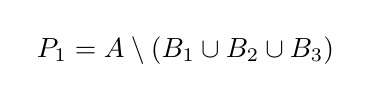
\begin{tikzpicture}[scale=4]
\PolygonP
\Trous
\node at (0.5,-0.05) {$P_1 = A \setminus \left(B_1 \cup B_2 \cup B_3\right)$};
\end{tikzpicture}

% \begin{tikzpicture}[scale=4]
% \PolygonP
% \Trous
% \end{tikzpicture}

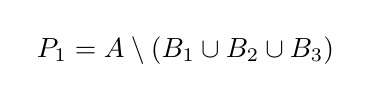
\begin{tikzpicture}[scale=4]
\Trous
\node at (0.5,-0.05) {$P_1 = A \setminus \left(B_1 \cup B_2 \cup B_3\right)$};
\end{tikzpicture}

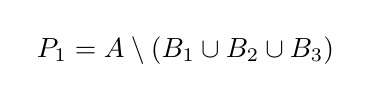
\begin{tikzpicture}[scale=4]
\TrouBDEUX
\node at (0.5,-0.05) {$P_1 = A \setminus \left(B_1 \cup B_2 \cup B_3\right)$};
\end{tikzpicture}

% \begin{tikzpicture}[scale=4]
% \TrouBUN
% \end{tikzpicture}

% \begin{tikzpicture}[scale=4]
% \TrouBTROIS
% \end{tikzpicture}

% \begin{tikzpicture}[scale=4]
% \TrouBDEUX
% \end{tikzpicture}

\begin{tikzpicture}[scale=4]
\ConvexHullBDEUX
\end{tikzpicture}

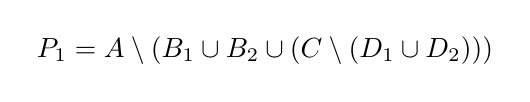
\begin{tikzpicture}[scale=4]
\TrouBDEUX
\TrousConvexHullBDEUXA
\TrousConvexHullBDEUXB
\node at (0.5,-0.05) {$P_1 = A \setminus \left(B_1 \cup B_2 \cup \left(C \setminus \left(D_1 \cup D_2\right)\right)\right)$};
\end{tikzpicture}

% \begin{tikzpicture}[scale=4]
% \TrousConvexHullBDEUXA
% \end{tikzpicture}

% \begin{tikzpicture}[scale=4]
% \TrousConvexHullBDEUXB
% \end{tikzpicture}

\end{document}